\documentclass[]{book}
\usepackage{lmodern}
\usepackage{amssymb,amsmath}
\usepackage{ifxetex,ifluatex}
\usepackage{fixltx2e} % provides \textsubscript
\ifnum 0\ifxetex 1\fi\ifluatex 1\fi=0 % if pdftex
  \usepackage[T1]{fontenc}
  \usepackage[utf8]{inputenc}
\else % if luatex or xelatex
  \ifxetex
    \usepackage{mathspec}
  \else
    \usepackage{fontspec}
  \fi
  \defaultfontfeatures{Ligatures=TeX,Scale=MatchLowercase}
\fi
% use upquote if available, for straight quotes in verbatim environments
\IfFileExists{upquote.sty}{\usepackage{upquote}}{}
% use microtype if available
\IfFileExists{microtype.sty}{%
\usepackage{microtype}
\UseMicrotypeSet[protrusion]{basicmath} % disable protrusion for tt fonts
}{}
\usepackage[margin=1in]{geometry}
\usepackage{hyperref}
\hypersetup{unicode=true,
            pdftitle={Case Studies in Reproducible Research: a spring seminar at UCSC},
            pdfauthor={Eric C. Anderson, Kristen C. Ruegg, Tina Cheng, and the students of EEB 295},
            pdfborder={0 0 0},
            breaklinks=true}
\urlstyle{same}  % don't use monospace font for urls
\usepackage{natbib}
\bibliographystyle{apalike}
\usepackage{color}
\usepackage{fancyvrb}
\newcommand{\VerbBar}{|}
\newcommand{\VERB}{\Verb[commandchars=\\\{\}]}
\DefineVerbatimEnvironment{Highlighting}{Verbatim}{commandchars=\\\{\}}
% Add ',fontsize=\small' for more characters per line
\usepackage{framed}
\definecolor{shadecolor}{RGB}{248,248,248}
\newenvironment{Shaded}{\begin{snugshade}}{\end{snugshade}}
\newcommand{\KeywordTok}[1]{\textcolor[rgb]{0.13,0.29,0.53}{\textbf{{#1}}}}
\newcommand{\DataTypeTok}[1]{\textcolor[rgb]{0.13,0.29,0.53}{{#1}}}
\newcommand{\DecValTok}[1]{\textcolor[rgb]{0.00,0.00,0.81}{{#1}}}
\newcommand{\BaseNTok}[1]{\textcolor[rgb]{0.00,0.00,0.81}{{#1}}}
\newcommand{\FloatTok}[1]{\textcolor[rgb]{0.00,0.00,0.81}{{#1}}}
\newcommand{\ConstantTok}[1]{\textcolor[rgb]{0.00,0.00,0.00}{{#1}}}
\newcommand{\CharTok}[1]{\textcolor[rgb]{0.31,0.60,0.02}{{#1}}}
\newcommand{\SpecialCharTok}[1]{\textcolor[rgb]{0.00,0.00,0.00}{{#1}}}
\newcommand{\StringTok}[1]{\textcolor[rgb]{0.31,0.60,0.02}{{#1}}}
\newcommand{\VerbatimStringTok}[1]{\textcolor[rgb]{0.31,0.60,0.02}{{#1}}}
\newcommand{\SpecialStringTok}[1]{\textcolor[rgb]{0.31,0.60,0.02}{{#1}}}
\newcommand{\ImportTok}[1]{{#1}}
\newcommand{\CommentTok}[1]{\textcolor[rgb]{0.56,0.35,0.01}{\textit{{#1}}}}
\newcommand{\DocumentationTok}[1]{\textcolor[rgb]{0.56,0.35,0.01}{\textbf{\textit{{#1}}}}}
\newcommand{\AnnotationTok}[1]{\textcolor[rgb]{0.56,0.35,0.01}{\textbf{\textit{{#1}}}}}
\newcommand{\CommentVarTok}[1]{\textcolor[rgb]{0.56,0.35,0.01}{\textbf{\textit{{#1}}}}}
\newcommand{\OtherTok}[1]{\textcolor[rgb]{0.56,0.35,0.01}{{#1}}}
\newcommand{\FunctionTok}[1]{\textcolor[rgb]{0.00,0.00,0.00}{{#1}}}
\newcommand{\VariableTok}[1]{\textcolor[rgb]{0.00,0.00,0.00}{{#1}}}
\newcommand{\ControlFlowTok}[1]{\textcolor[rgb]{0.13,0.29,0.53}{\textbf{{#1}}}}
\newcommand{\OperatorTok}[1]{\textcolor[rgb]{0.81,0.36,0.00}{\textbf{{#1}}}}
\newcommand{\BuiltInTok}[1]{{#1}}
\newcommand{\ExtensionTok}[1]{{#1}}
\newcommand{\PreprocessorTok}[1]{\textcolor[rgb]{0.56,0.35,0.01}{\textit{{#1}}}}
\newcommand{\AttributeTok}[1]{\textcolor[rgb]{0.77,0.63,0.00}{{#1}}}
\newcommand{\RegionMarkerTok}[1]{{#1}}
\newcommand{\InformationTok}[1]{\textcolor[rgb]{0.56,0.35,0.01}{\textbf{\textit{{#1}}}}}
\newcommand{\WarningTok}[1]{\textcolor[rgb]{0.56,0.35,0.01}{\textbf{\textit{{#1}}}}}
\newcommand{\AlertTok}[1]{\textcolor[rgb]{0.94,0.16,0.16}{{#1}}}
\newcommand{\ErrorTok}[1]{\textcolor[rgb]{0.64,0.00,0.00}{\textbf{{#1}}}}
\newcommand{\NormalTok}[1]{{#1}}
\usepackage{longtable,booktabs}
\usepackage{graphicx,grffile}
\makeatletter
\def\maxwidth{\ifdim\Gin@nat@width>\linewidth\linewidth\else\Gin@nat@width\fi}
\def\maxheight{\ifdim\Gin@nat@height>\textheight\textheight\else\Gin@nat@height\fi}
\makeatother
% Scale images if necessary, so that they will not overflow the page
% margins by default, and it is still possible to overwrite the defaults
% using explicit options in \includegraphics[width, height, ...]{}
\setkeys{Gin}{width=\maxwidth,height=\maxheight,keepaspectratio}
\IfFileExists{parskip.sty}{%
\usepackage{parskip}
}{% else
\setlength{\parindent}{0pt}
\setlength{\parskip}{6pt plus 2pt minus 1pt}
}
\setlength{\emergencystretch}{3em}  % prevent overfull lines
\providecommand{\tightlist}{%
  \setlength{\itemsep}{0pt}\setlength{\parskip}{0pt}}
\setcounter{secnumdepth}{5}
% Redefines (sub)paragraphs to behave more like sections
\ifx\paragraph\undefined\else
\let\oldparagraph\paragraph
\renewcommand{\paragraph}[1]{\oldparagraph{#1}\mbox{}}
\fi
\ifx\subparagraph\undefined\else
\let\oldsubparagraph\subparagraph
\renewcommand{\subparagraph}[1]{\oldsubparagraph{#1}\mbox{}}
\fi

%%% Use protect on footnotes to avoid problems with footnotes in titles
\let\rmarkdownfootnote\footnote%
\def\footnote{\protect\rmarkdownfootnote}

%%% Change title format to be more compact
\usepackage{titling}

% Create subtitle command for use in maketitle
\newcommand{\subtitle}[1]{
  \posttitle{
    \begin{center}\large#1\end{center}
    }
}

\setlength{\droptitle}{-2em}
  \title{Case Studies in Reproducible Research: a spring seminar at UCSC}
  \pretitle{\vspace{\droptitle}\centering\huge}
  \posttitle{\par}
  \author{Eric C. Anderson, Kristen C. Ruegg, Tina Cheng, and the students of EEB
295}
  \preauthor{\centering\large\emph}
  \postauthor{\par}
  \predate{\centering\large\emph}
  \postdate{\par}
  \date{2017-03-23}

\usepackage{booktabs}
\usepackage{amsthm}
\makeatletter
\def\thm@space@setup{%
  \thm@preskip=8pt plus 2pt minus 4pt
  \thm@postskip=\thm@preskip
}
\makeatother

\usepackage{amsthm}
\newtheorem{theorem}{Theorem}[chapter]
\newtheorem{lemma}{Lemma}[chapter]
\theoremstyle{definition}
\newtheorem{definition}{Definition}[chapter]
\newtheorem{corollary}{Corollary}[chapter]
\newtheorem{proposition}{Proposition}[chapter]
\theoremstyle{definition}
\newtheorem{example}{Example}[chapter]
\theoremstyle{remark}
\newtheorem*{remark}{Remark}
\begin{document}
\maketitle

{
\setcounter{tocdepth}{1}
\tableofcontents
}
\chapter{Course Overview}\label{course-overview}

This is the home for the lecture notes for a proposed course in data
analysis and reproducible research using R, Rstudio, and GitHub.

The seminar is called, ``Case Studies in Reproducible Research,'' but we
utter that title with the caveat that, although the organizers have
quite a few case studies that they could spin up for this course, the
case studies we will be studying in this course are going to be actual
research projects that the participants are working on. You're gonna
bring 'em, and we are going to collectively help you wrassle them into a
reasonable and reproducible data analysis. In the process we will touch
on a number of elements of data analysis with R.

For the interested, these materials were all prepared using RStudio's
\href{https://bookdown.org/}{bookdown} package.

\section{The origin of this seminar}\label{the-origin-of-this-seminar}

The idea for this course was floated by Tina Cheng who was planning to
lead a seminar in spring 2017 based in part on Eric C. Anderson's
\href{http://eriqande.github.io/rep-res-web/}{``Reproducible Research
Course''}, taught at the Southwest Fisheries Science Center in the fall
of 2014. Although going over those notes might have been a reasonable
exercise, it turns out that a lot has changed in the world of data
analysis since fall 2014, and the notes from that course are, today, a
little bit dated.

We have been particularly excited by the ascendancy of Hadley Wickham's
\href{http://tidyverse.org/}{Tidyverse} approach to data analysis, and
the tremendous development of a variety of tools developed by
\href{https://www.rstudio.com/}{RStudio} for integrating report
generation and data analysis into reproducible workflows. In fact, Eric
has been saying for the last year that if he were to teach another
course on data analysis it would be structured completely differently
than his \href{http://eriqande.github.io/rep-res-web/}{``Reproducible
Research Course''}. So, it was clearly time for him to stop talking and
help put together an updated and different course.

At the same time, in working on our own projects and in helping others,
we have consistently found that the most effective way for anyone to
learn data analysis is to ensure that it is immediately relevant to
whatever ongoing research project is currently consuming them.
Therefore, in the current seminar, we are hoping to spend at least half
of our time ``workshopping'' the data sets that seminar participants are
actually involved in analyzing. Together we will help students wrestle
their data, analyses, and ideas into a single, well-organized RStudio
project under version control with git. Therefore, every student should
come to this course with a data set and an associated analysis project.
This is also not a ``first course in R''. Student coming to the course
should have at least a little familiarity with using R.

\section{Course Organizers}\label{course-organizers}

\begin{description}
\item[Kristen C. Ruegg]
We can put description here
\item[Eric C. Anderson]
We can put more description here.
\item[Tina Cheng]
something here
\end{description}

\section{Course Goals}\label{course-goals}

The goal of this course is for scientists, researchers, and students to
learn to:

\begin{itemize}
\tightlist
\item
  properly store, manage, and distribute their data in a \emph{tidy}
  format
\item
  consolidate their digital research materials and analyses into
  well-organized RStudio projects.
\item
  use the tools of the tidyverse to manipulate and analyze those data
  sets
\item
  integrate data analysis with report generation and article preparation
  using the Rmarkdown format and using
  \href{http://rmarkdown.rstudio.com/r_notebooks.html}{R Notebooks}
\item
  use git version control software and GitHub to effectively manage data
  and source code, collaborate efficiently with other researchers, and
  neatly package their research.
\end{itemize}

By the end of the course, the hope is that we will all have mastered
strategies allowing us to use the above-listed, freely-available and
open-source tools for conducting research in a reproducible fashion. The
ideal we will be striving for is to be able to start from a raw data set
and then write a computer program that conducts all the cleaning,
manipulation, and analysis of the data, and presentation of the results,
in an automated fashion. Carrying out analysis and report-generation in
this way carries a number of advantages to the researcher:

\begin{enumerate}
\def\labelenumi{\arabic{enumi}.}
\tightlist
\item
  Newly-collected data can be integrated easily into your analysis.
\item
  If a mistake is found in one section of your analysis, it is not
  terribly onerous to correct it and then re-run all the downstream
  analyses.
\item
  Revising a manuscript to address referee comments can be done quickly.
\item
  Years after publication, the exact steps taken to analyze the data
  will still be available should anyone ask you how, exactly, you did an
  analysis!
\item
  If you have to conduct similar analyses and produce similar reports on
  a regular bias with new data each time, you might be able to do this
  readily by merely updating your data and then automatically producing
  the entire report.
\item
  If someone finds an error in your work, they can fix it and then
  easily show you exactly what they did to fix it.
\end{enumerate}

Additionally, packaging one's research in a reproducible fashion is
beneficial to the research community. Others that would like to confirm
your results can do so easily. If someone has concerns about exactly how
a particular analysis was carried out, they can find the precise details
in the code that you wrote to do it. Someone wanting to apply your
methods to their own data can easily do so, and, finally, if we are all
transparent and open about the methods that we use, then everyone can
learn more quickly from their colleagues.

In many fields today, publication of research requires the submission of
the original data to a publicly-available data repository. Currently,
several journals require that all analyses be packaged in a clear and
transparent fashion for easy reproduction of the results, and I predict
that trend will continue until most, if not all, journals will require
that data analyses be available in easily reproduced formats. This
course will help scientists prepare themselves for this eventuality. In
the process, you will probably find that conducting your research in a
reproducible fashion helps you work more efficiently (and perhaps even
more enjoyably!)

\section{Weekly Syllabus}\label{weekly-syllabus}

\begin{description}
\item[Week 1 --- Get Your Workspace Set Up]
Eric and Kristen will be absent
\item[Week 2 --- RStudio project organization tips]
something something
\item[Week 3 --- git down with it! Interfacing with git and GitHub]
something something description
\end{description}

\chapter{Applications}\label{applications}

Some \emph{significant} applications are demonstrated in this chapter.

\section{Example one}\label{example-one}

\section{Example two}\label{example-two}

You can label chapter and section titles using \texttt{\{\#label\}}
after them, e.g., we can reference Chapter \ref{intro}. If you do not
manually label them, there will be automatic labels anyway, e.g.,
Chapter \ref{methods}.

Figures and tables with captions will be placed in \texttt{figure} and
\texttt{table} environments, respectively.

\begin{Shaded}
\begin{Highlighting}[]
\KeywordTok{par}\NormalTok{(}\DataTypeTok{mar =} \KeywordTok{c}\NormalTok{(}\DecValTok{4}\NormalTok{, }\DecValTok{4}\NormalTok{, .}\DecValTok{1}\NormalTok{, .}\DecValTok{1}\NormalTok{))}
\KeywordTok{plot}\NormalTok{(pressure, }\DataTypeTok{type =} \StringTok{'b'}\NormalTok{, }\DataTypeTok{pch =} \DecValTok{19}\NormalTok{)}
\end{Highlighting}
\end{Shaded}

\begin{figure}

{\centering 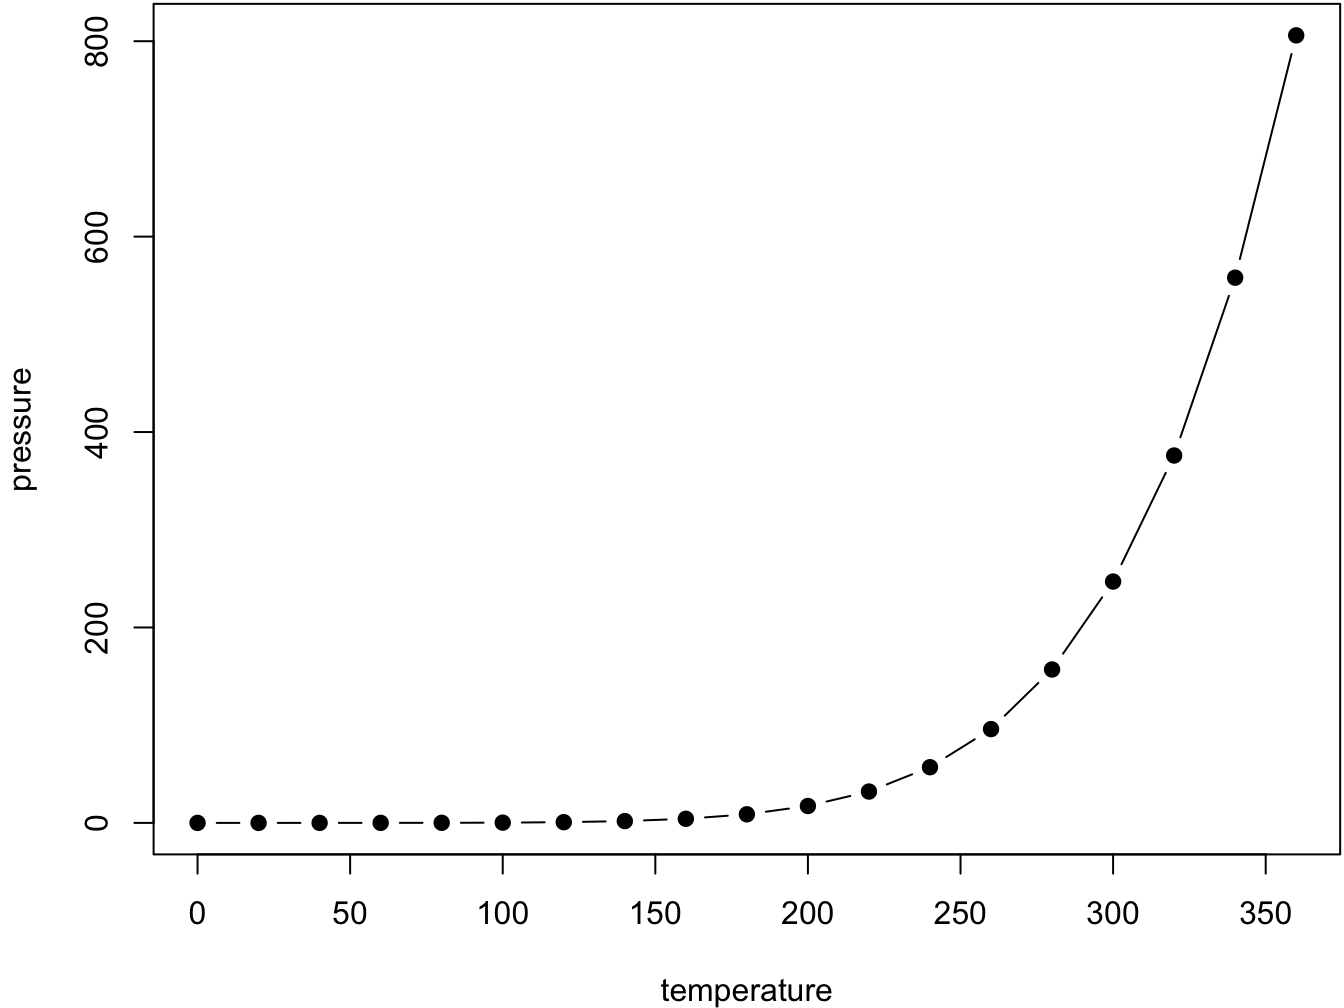
\includegraphics[width=0.8\linewidth]{bookdown-demo_files/figure-latex/nice-fig-1} 

}

\caption{Here is a nice figure!}\label{fig:nice-fig}
\end{figure}

Reference a figure by its code chunk label with the \texttt{fig:}
prefix, e.g., see Figure \ref{fig:nice-fig}. Similarly, you can
reference tables generated from \texttt{knitr::kable()}, e.g., see Table
\ref{tab:nice-tab}.

\begin{Shaded}
\begin{Highlighting}[]
\NormalTok{knitr::}\KeywordTok{kable}\NormalTok{(}
  \KeywordTok{head}\NormalTok{(iris, }\DecValTok{20}\NormalTok{), }\DataTypeTok{caption =} \StringTok{'Here is a nice table!'}\NormalTok{,}
  \DataTypeTok{booktabs =} \OtherTok{TRUE}
\NormalTok{)}
\end{Highlighting}
\end{Shaded}

\begin{table}

\caption{\label{tab:nice-tab}Here is a nice table!}
\centering
\begin{tabular}[t]{rrrrl}
\toprule
Sepal.Length & Sepal.Width & Petal.Length & Petal.Width & Species\\
\midrule
5.1 & 3.5 & 1.4 & 0.2 & setosa\\
4.9 & 3.0 & 1.4 & 0.2 & setosa\\
4.7 & 3.2 & 1.3 & 0.2 & setosa\\
4.6 & 3.1 & 1.5 & 0.2 & setosa\\
5.0 & 3.6 & 1.4 & 0.2 & setosa\\
\addlinespace
5.4 & 3.9 & 1.7 & 0.4 & setosa\\
4.6 & 3.4 & 1.4 & 0.3 & setosa\\
5.0 & 3.4 & 1.5 & 0.2 & setosa\\
4.4 & 2.9 & 1.4 & 0.2 & setosa\\
4.9 & 3.1 & 1.5 & 0.1 & setosa\\
\addlinespace
5.4 & 3.7 & 1.5 & 0.2 & setosa\\
4.8 & 3.4 & 1.6 & 0.2 & setosa\\
4.8 & 3.0 & 1.4 & 0.1 & setosa\\
4.3 & 3.0 & 1.1 & 0.1 & setosa\\
5.8 & 4.0 & 1.2 & 0.2 & setosa\\
\addlinespace
5.7 & 4.4 & 1.5 & 0.4 & setosa\\
5.4 & 3.9 & 1.3 & 0.4 & setosa\\
5.1 & 3.5 & 1.4 & 0.3 & setosa\\
5.7 & 3.8 & 1.7 & 0.3 & setosa\\
5.1 & 3.8 & 1.5 & 0.3 & setosa\\
\bottomrule
\end{tabular}
\end{table}

You can write citations, too. For example, we are using the
\textbf{bookdown} package \citep{R-bookdown} in this sample book, which
was built on top of R Markdown and \textbf{knitr} \citep{xie2015}.

\bibliography{packages.bib,book.bib}


\end{document}
